\documentclass[tikz,border=8pt]{standalone}
% Shared look for every TikZ diagram. Load with \input{../../tools/tikz-style.tex}
\usepackage[T1]{fontenc}
\usepackage{lmodern}
\renewcommand{\sfdefault}{lmr}  % diagrams use the same serif as the text
\usetikzlibrary{arrows.meta, positioning, shapes.geometric, calc, fit, backgrounds}
\definecolor{cblue}{HTML}{4C78A8}
\definecolor{corange}{HTML}{F58518}
\definecolor{cgreen}{HTML}{54A24B}
\definecolor{cred}{HTML}{E45756}
\definecolor{cpurple}{HTML}{B279A2}
\definecolor{cgrey}{HTML}{6B6B6B}
\tikzset{
  every picture/.style={font=\sffamily, line width=1.2pt},
  box/.style={draw=#1, fill=#1!12, rounded corners=4pt, align=center, inner sep=7pt, minimum height=1.1cm},
  box/.default=cgrey,
  arrow/.style={-{Stealth[length=3mm]}, draw=cgrey, line width=1.4pt},
  title/.style={font=\sffamily\bfseries\Large},
  note/.style={font=\sffamily\small, text=cgrey, align=center},
}
\AtBeginDocument{\hyphenpenalty=10000 \exhyphenpenalty=10000}

\begin{document}
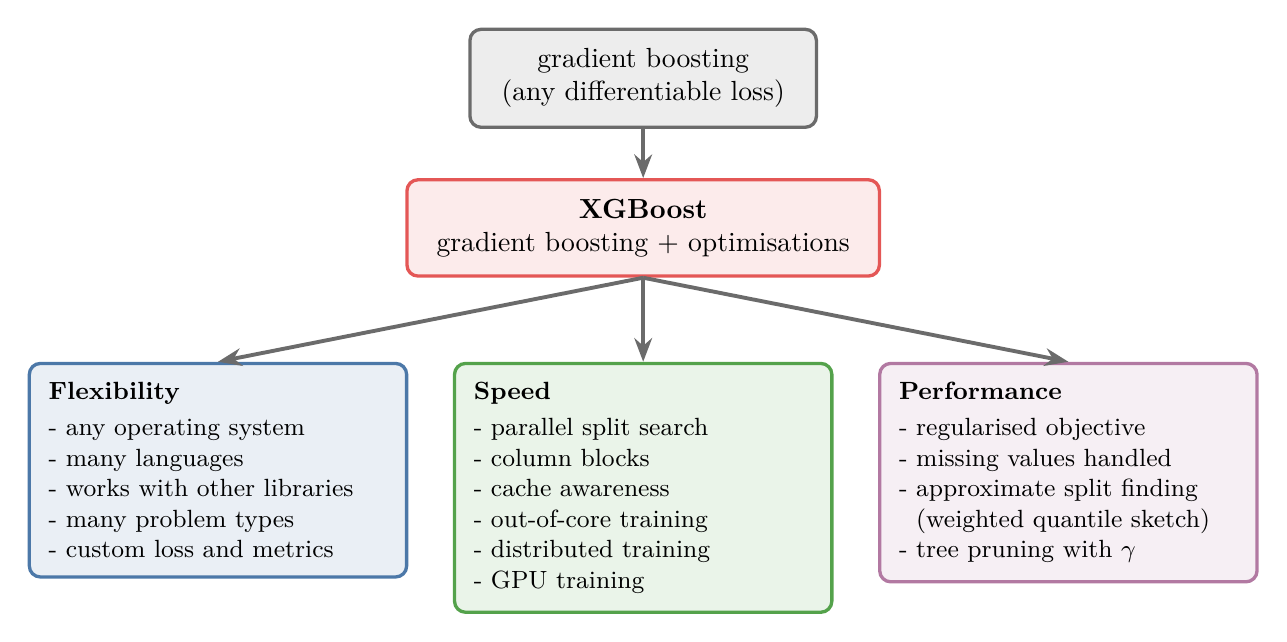
\begin{tikzpicture}[a/.style={box=#1, minimum width=4.6cm, align=left, text width=4.3cm, font=\sffamily\small}]
  \node[box=cred, minimum width=6cm] (x) at (0,0) {\textbf{XGBoost}\\gradient boosting + optimisations};
  \node[box=cgrey, minimum width=4.4cm] (gb) at (0,1.9) {gradient boosting\\(any differentiable loss)};
  \draw[arrow] (gb) -- (x);
  \node[a=cblue, anchor=north] (f) at (-5.4,-1.7) {\textbf{Flexibility}\\[2pt]
    - any operating system\\- many languages\\- works with other libraries\\- many problem types\\- custom loss and metrics};
  \node[a=cgreen, anchor=north] (s) at (0,-1.7) {\textbf{Speed}\\[2pt]
    - parallel split search\\- column blocks\\- cache awareness\\- out-of-core training\\- distributed training\\- GPU training};
  \node[a=cpurple, anchor=north] (p) at (5.4,-1.7) {\textbf{Performance}\\[2pt]
    - regularised objective\\- missing values handled\\- approximate split finding\\\ \ (weighted quantile sketch)\\- tree pruning with $\gamma$};
  \draw[arrow] (x.south) -- (f.north); \draw[arrow] (x) -- (s); \draw[arrow] (x.south) -- (p.north);
\end{tikzpicture}
\end{document}
